%!TEX root = ../Thesis.tex

In this chapter, we introduce Gene Set Enrichment Analysis as a powerful tool for the analysis and interpretation of large-scale biological data. We first descibe the algorithm for enrichment analysis in details, more specifically the Running Sum Statistic. Later, we present two methods for computing p-values for enrichment analysis, while providing the appropriate background information on statistical hypothesis testing.

\section{Enrichment Analysis}\label{sec:enrichment}

\subsection{Motivation}\label{subsec:ea_motivation}
In this thesis, we want to identify molecular properties of cancer cells (e.g.\ gene or pathway expression) which are particularly associated with an increased sensitivity or resistance to a specific drug.\\
For this, we use the analytical method of \textbf{Gene Set Enrichment Analysis} (GSEA), as introduced by Subramanian et al.\ in 2005~\cite{gsea_original}. Originally, this method was developed to characterize differential gene expression of pathways between different cancer patients, or between healthy and cancer patients. While the previous gene expression analysis on individual genes isn't able to find much similarity between patients, GSEA was able to reveal many common pathways~\cite{gsea_original}.\\
While this is what GSEA was originally designed and developed for, since it is in itself a purely mathematical method, it presents great flexibility for applying it to significantly different types of input data. GSEA allows us to assess whether biological entities that have a certain property are significantly accumulated at the beginning or the end of a sorted list, so in other words, whether that biological property is associated with a rather low or high value of the measure by which the list was sorted.\\
The potential applications are vast: the sorted list can describe genes and their expression values, with the respective categories describing gene sets corresponding to pathways and the genes that are part of those pathways, but the sorted list could also describe all kinds of other biological entities. For example, in this thesis, we will consider cancer cell lines sorted by a drug sensitivity value, with the respective categories describing any biological property characterizing these cell lines, like gene common expression alterations, mutations, or any other property which applies to some, but not all, cell lines.\\
Different approaches and improvements on GSEA have been implemented since the original inception of the method. \textbf{GeneTrail}~\cite{genetrail}, published by Backes et.\ al.\ in 2007, is a framework providing GSEA as one of its features, which is available as a web service.\\
There are two slightly different variants of Gene Set Enrichment Analysis, namely a weighted variant (WGSEA) and an unweighted variant~\cite{gsea_original}. For the purpose of this thesis, we will be focusing on Unweighted Gene Set Enrichment Analysis.

%Since the completion of the Human Genome Project in 2003, DNA sequencing methods have undergone substantial advancements. While it took 13 years to initially sequence the human genome, nowadays, new methods such as DNA microarrays, next-generation sequencing and other widely available and cheap technologies for genome sequencing and analysis have transformed the landscape of research: the challenges faced by researchers have been shifted from the acquisition of data to the interpretation of said data, to gain biological insights.
%As a basis for these analyses, researchers work with a ranked list of genes, sorted by differential expression.\\
%In previous approaches, genes at the beginning or end of the list were deemed as significantly over- or underexpressed, and attempted to discern biological properties common to these genes, to make biological statements about the differential expression of those genes.
%This approach, however, faces several analytical challenges, including but not limited to, the number of genes declared significant being either much to large or much too small to make meaningful statments.
%Additionally, this type of analysis is only able to focus on individual genes, which biologically speaking is not meaningful, since biological processes are controlled by pathways involving many genes.\\
%One approach developed to counteract these problems, originally introduced in 2005 by Subramarian et al., is called \textbf{Gene Set Enrichment Analysis}~\cite{gsea_original}.
%It produces more significiant and biologically interesting results since it uses gene sets (which represent previous biological knowledge) instead of individual genes.\\

%\subsection{Input values for GSEA}

%In other words, we want to assess whether the category $C$ (which could, for example, represent a pathway) is linked to interestingly high or low gene expression.\\
%$C = \{l_a, l_b, \ldots\}$ \todo{formulation not clean}(with $1 \leq a \leq b \leq \cdots \leq n$)
%This\todo{repeat with the previous section. decide which one to keep} kind of analysis can also be applied to several other types of input data. For instance, the datatypes we started our analyses with were lists of cancer cell lines, sorted by their respective sensitivity to a certain drug, expressed as an IC50 value. As a category, we use gene expression alterations which have been cataloged by researchers over time, or determined based on gene expression data taken from widely available databases. The result of this enrichment analysis would then be a way to statistically link gene expression alterations present in cancer cell lines to an especially high sensitivity or resistance to a specific drug.\\
%The same enrichment analysis can also be performed by replacing the gene expression alteration categories by arbitrary biological features present in some, but not all cancer cell lines. Those features can then be linked up to notable drug sensitivty or resistance by performing GSEA.\\

\subsection{GSEA and Running Sum Statistic}\label{subsec:ea_gsea_rss}
%The main step of Gene Set Enrichment Analysis is to perform a running sum statistic.\\
Considering the starting point of a list of entities $L = l_1, l_2, \ldots, l_n$ sorted by a biological measurement, Gene Set Enrichment Analysis assesses for a biological category $C$ containing $j$ members of $L$, if the elements of $C$ are accumulated significantly at the beginning or the end of the sorted list. It does that by computing a running sum statistic on the the list $L$.\\
For now, we will abstract away from the concrete applications and explore the running sum statistic as a pure mathematical concept. After that, we will come back to the concrete data and show the actual proceeding for performing a running sum statistic in Gene Set Enrichment Analysis.\\
To perform such a running sum statistic for Unweighted Gene Set Enrichment Analysis, we need two things: on the one hand, a sorted list of values, and on the other hand, a category which encompasses some, but not all of the objects belonging to the values in our list. Our goal is to assess whether the values contained in the category are accumulated at the beginning or the end of the list.\\
We proceed to go through the list from top to bottom. Consider a list with $n$ objects, $j$ of which are in the category we are considering.\\
The running sum statistic $RS$ is started at a value of $0$~\cite{genetrail_original}:
\begin{align}
RS(0)&=0
\end{align}
For every further element $1 \leq k \leq n$, we consider~\cite{genetrail_original}:
\begin{align}
RS(k)&=\begin{cases}
	RS(k-1)+(n-j)& \text{if }l_{k}\in C\\
	RS(k-1)-j&\text{else}
\end{cases}
\end{align}
For every element belonging to the category $C$, we increase the running sum by $n-l$. For every element not in the category $C$, we decrease the running sum by $l$.\\
Note that the running sum is constructed in such a way that it always ends at $0$:
\begin{align}
	RS(n) = l*(n-l)+(n-l)*(-l) = 0
\end{align}
One such list could look like this:\\
\begin{tabular}{m{1.5em} m{1.5em} m{1.5em} m{1.5em} m{1.5em} m{1.5em} m{1.5em} m{1.5em} m{1.5em} m{1.5em}}
	\color{Cerulean}0.2&
	\color{Cerulean}0.3&
	\color{Black}0.4&
	\color{Cerulean}0.45&
	\color{Black}0.47&
	\color{Cerulean}0.48&
	\color{Black}0.6&
	\color{Black}0.65&
	\color{Black}0.7&
	\color{black}0.71
\end{tabular}\\
Here, the blue numbers represent the entries that belong to our category $C$.\\
Applying this running sum statistic to the example list presented above, we get the following values: $n=10$, $l$=$4$, and $n-l=6$.\\
The running sum for the list above can be seen in Table~\ref{table:rss} as well as in Figure~\ref{fig:rss}.\\
\begin{table}
	\centering
	\begin{tabular}{|c|c|c|}
		\hline
		Step&Value&RSS\\
		\hline
		0&&0\\
		\hline
		1&\color{Cerulean}0.2\color{Black}&6\\
		\hline
		2&\color{Cerulean}0.3\color{Black}&12\\
		\hline
		3&0.4&8\\
		\hline
		4&\color{Cerulean}0.45\color{Black}&14\\
		\hline
		5&0.47&10\\
		\hline
		6&\color{Cerulean}0.48\color{Black}&\color{WildStrawberry}16\color{Black}\\
		\hline
		7&0.6&12\\
		\hline
		8&0.65&8\\
		\hline
		9&0.7&4\\
		\hline
		10&0.71&0\\
		\hline
	\end{tabular}
	\caption{Running Sum Statistic in table form}
	\label{table:rss}
\end{table}\\
The value of interest used for characterizing the level and direction of the enrichment is the maximum deviation from $0$ reached by the running sum. This value is designated the \emph{enrichment score} and denoted $RS_{C}$.\\
The maximum deviation from $0$ in this concrete case is $16$, which is highlighted in red in the graph in Figure~\ref{fig:rss}.\\
The absolute value of the enrichment score gives a rough measure of the strength of the enrichment, though the specific methods for significance estimation (c.f.\ \textit{p-values}) will be discussed later. The sign of the maximum deviation tells us the direction of the enrichment: a positive score means that the values contained in the category are accumulated at the beginning of the list (the category is \textit{enriched} at the beginning of the list), while a negative scores means that the values are accumulated at the end of the list (the category is \textit{depleted} at the beginning of the list, or accumulated at the end of the list).
\begin{figure}
	\centering
	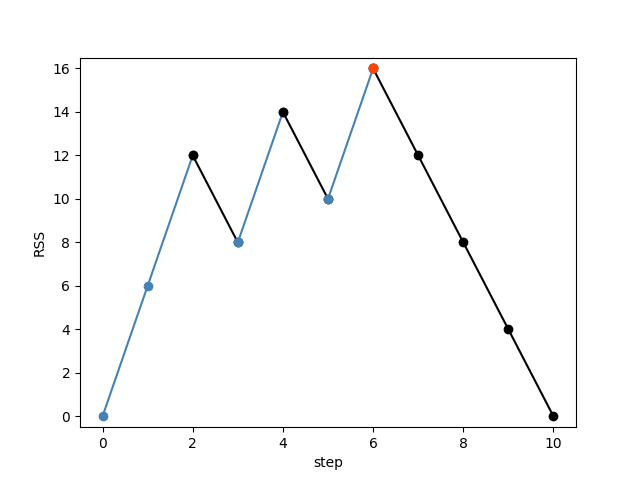
\includegraphics[width=0.9\textwidth]{rss_highlight.png}
	\caption{Running Sum Statistic in graph form}
	\label{fig:rss}
\end{figure}

\subsection{Interpretation Example}\label{subsec:ea_example}
As mentioned previously, this method of the running sum statistic can be applied with numerous types of data used as sorted list and category respectively.\\
One such application scenario, which will be executed and discussed in detail later on, is the following scenario:
\begin{itemize}
	\item the sorted list contains drug sensitivity values for cancer cell lines for one specific drug, e.g.\ $IC_{50}$ values. They are sorted from low $IC_{50}$ (which signifies a strong sensitivity to the drug) to high $IC_{50}$ (which indicates a strong resistance).
	\item the categories consider known gene expression alterations for our cell lines. The specific up- or down-regulation of a single gene constitutes a category, with every cell line known to have this alteration being considered part of the category.
\end{itemize}
After performing the running sum statistic, we might notice that the category might be accumulated at the beginning of the sorted list, as indicated by a positive enrichment score. This indicates that the concrete gene expression alteration that was used as a category is linked to a lower $IC_{50}$ value, or a stronger sensitivity to the considered drug.\\
Of course, this is only an indication of statistical correlation and does not imply any causation. Still, it can provide a great starting point for future analyses.\\
The magnitude of that statistical association is in some way expressed by the enrichment score. However, to make independently interpretable and comparable statements about this statistical association, we need to be able to provide \emph{p-values}.

\section{p-Value Computation}\label{sec:p-value}

%As for most scientific processes involving predictions, our results have no value without a measure of statistical significance in the form of a \emph{p-value} attached to them.
The enrichment scores provided by the running sum statistic allow us to compare different results to a certain extent, and to estimate if the accumulation is rather at the beginning or the end of the list. However, to truly quantify the significance of the accumulation, we need to provide \emph{p-values} for our results.\\
In statistics, a \emph{hypothesis test} is a method of statistical inference used to determine whether a sample of data sufficiently supports a particular hypothesis to be true for the entire population~\cite{statistics_moore}. The \emph{null hypothesis} $H_0$ typically represents the claim that the studied effect does not exist, and is initially assumed to be true. The \emph{alternative hypothesis} $H_1$ represents the claim that there is a significant effect occurring in the observed data.\\
For instance, considering the example application scenario in the previous section, the hypothesis test might be formulated as follows:
\begin{itemize}
	\item $H_0$: ``The over-expression of gene X \textbf{is not linked} to any increased sensitivity or resistance to drug Y''
	\item $H_1$: ``The over-expression of gene X \textbf{is linked} to an increased sensitivity or resistance to drug Y''
\end{itemize}
When we make a prediction, we can either make a correct prediction, or an error. Errors can either be Type I or Type II errors. A Type I error (false positive prediction) is when we reject the null hypothesis even though it is, in fact, true. A Type II error (false negative prediction) is when we do not reject the null hypothesis when, in fact, we should have rejected it~\cite{type1type2error}.\\
A \emph{p-value} is a value expressing statistical significance. Intuitively speaking, it describes the likeliness of a certain result having occurred purely by chance.
Mathematically speaking, the definition of a p-value is as follows: a p-value expresses the likelihood of obtaining a value at least as significant as the observed result if the null hypothesis $H_{0}$ is true~\cite{p-value_def}.\\
The smaller the p-value, the less likely it is that the result has occured purely by chance. However, to decide if a result should be considered significant or not is a binary decision. Thereby, we need to define a cut-off value for the p-value, for a result to be considered significant. Usually, that cut-off value is set to $p \leq 0.05$.\\
After discussing p-values generally, we will now see two methods for calculating p-values specifically for the GSEA method.

\subsection{Mehtod \Romannum{1}:\@Permutation Tests}\label{subsec:p-value-perm}
The originally proposed method for calculating p-values for an unweighted GSEA analysis involves the perform of so-called permutation tests.
Permutation tests involve generating a large number of random permutations of the elements in a list, while maintaining their associated categories. For each permutation, the running sum statistic is calculated, and the corresponding enrichment score is noted. Then, the enrichment score of the analysis we are trying to provide a p-value for is checked against the other calculated enrichment scores. The p-value is calculated based on the definition of a p-value: It is estimated by approximating the probability of obtaining a result at least as significant as the observed one occurring purely by chance. This probability is based on the proportion of such results seen in the simulations.
%it is approximated by calculating the likeliness of a result at least as significant as ours to be occuring purely by chance, based on the proportion of it occuring in our observations:
\begin{align}
\text{p-value} = \frac{\text{\# of running sums reaching at least the enrichment score to be assessed } +1 }{\text{\# of running sums simulated in total}}
\end{align}
The 1 in the numerator is added for practical reasons: If our enrichment score of interest is reached in none of our simulated runs, our method would return a p-value of $0$, which we want to avoid, as it would imply absolute certainty that the result (or a more extreme result) could never happen under the Null hypothesis (guarantee a link between drug sensitivity and gene expression, e.g.).
%However, this is not what our permutation tests would intuitively mean, since the p-value would increase eventually by performing more tests.
By adding 1, we return a very small p-value, which is consistent with what this p-value expresses.
%{\color{gray}
%As this is only an approximation of the actual p-value and not a precise calculation, we do not only want to provide a p-value, but also a value of how representative and reliable this p-value is, called \emph{representitativeness}.
%In our case, the resolution is the proportion of possible permutations for which a running sum statistic was simulated, which intuitively speaking represents the confidence we have in our estimation of the p-value\todo{find a source or just leave this measure unnamed}.\\
%\begin{align}
%	\text{representitativeness} = \frac{\text{\# of running sums simulated}}{\text{\# of possible running sums}} = \frac{\text{\# of running sums simulated}}{\binom{n}{l}}
%\end{align}
%}
This method calculates the p-value by its very definition: a p-value is the likeliness of a result being obtained purely by chance, and permutation tests generate random results and check if we reached our result of interest.\\
It has the advantage of being rather simple to understand and implement.\\
However, this method has a great price in performance as the number of possible permutations increases immensely with the length of the running sums occurring in practice. For instance, if we consider a list of 100 genes with 10 belonging to our considered category, the number of possible permutations is $\binom{100}{10}\approx10^{13}$. If we had a list of 1000 genes with 100 belonging to the category, the number of permutations would be $\binom{1000}{100}\approx10^{139}$.\\
As for most analyses in the field of bioinformatics and beyond, we are greatly interested in having the p-values attached to our results be as small as possible.\\
When performing $N$ permutation tests, the smallest achievable p-value is going to be $\frac{1}{N}$. In a way, permutations tests do not give an precise approximation for the p-value itself, but rather an approximation for an upper bound for the p-value. This, in combination with the limited resolution, requires us to simulate an extremely large number of permutations to get a desired low p-value, which implies significant computing power and time demands.\\
Another problem with permutation tests is that, due to the random sampling procedures, this method is inherently non-deterministic. This means that repeated runs may lead to different p-value estimations, which is evidently undesirable.

\subsection{Method \Romannum{2}: Precise p-value Computation}\label{subsec:p-value-precise}
\begin{table}
	\centering
	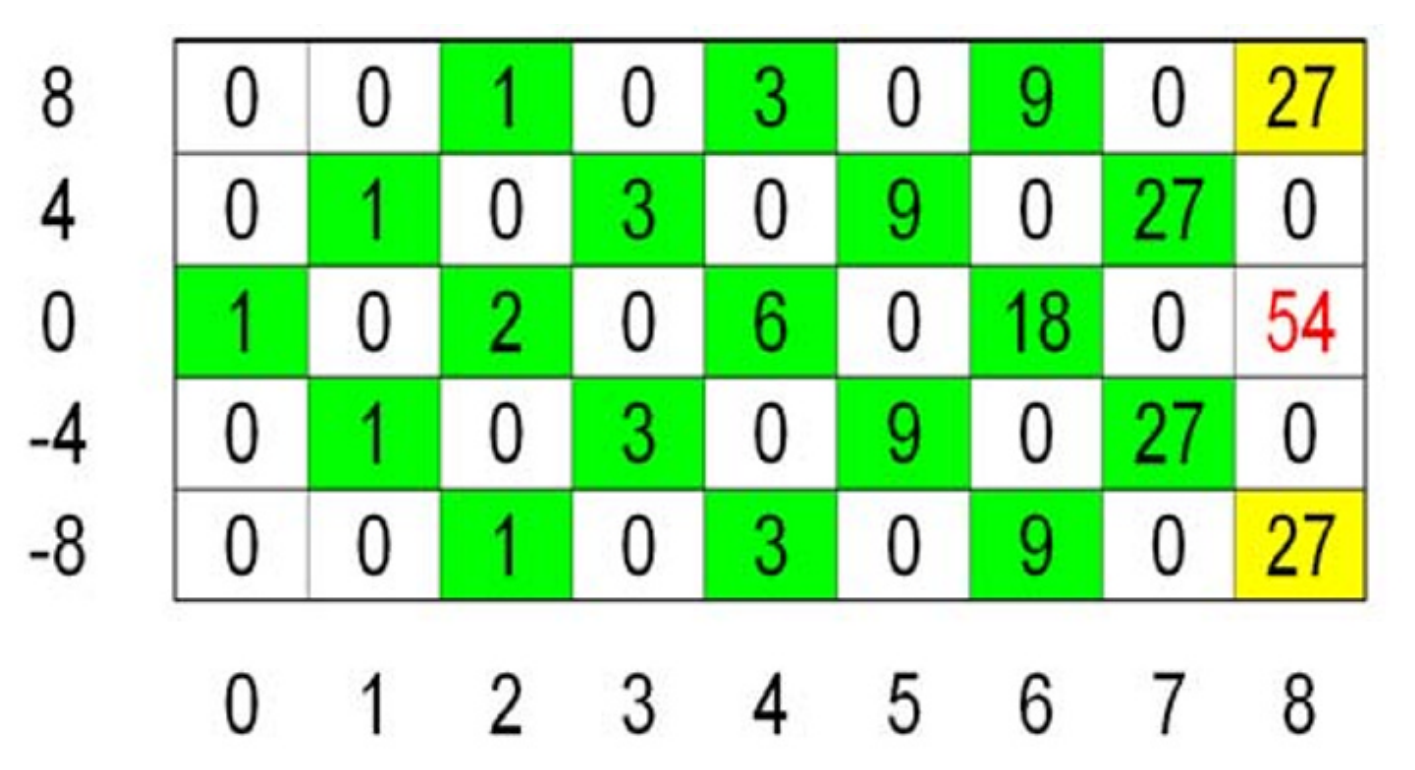
\includegraphics[width=0.9\textwidth]{dynamic_programming_matrix.png}
	\caption{Example dynamic programming matrix.\\We have a list of $8$ elements, of which $4$ are in the category. We consider $RS_{C}<12$.\\The states reached by our running sum are green, the yellow numbers can be discarded.\\Our final number of running sums which fulfill this is $54$.}
	\label{tab:matrix}
\end{table}
As the permutation tests are only able to provide approximate p-values, a method to calculate p-values precisely for unweighted GSEA is obviously very desirable. One such method, presented in the following, was introduced as an extension of the \textbf{GeneTrail} platform in 2007 by Keller et al.~\cite{genetrail_original, genetrail_dynamic_programming}\\
This precise p-value computation method utilizes a dynamic programming algorithm, where the number of running sum statistics reaching our maximum deviation value is counted in a dynamic programming matrix.\\
We calculate the probability of a random running sum reaching our value of interest $RS_{C}$ using the complement of the event as $1 - \frac{X}{Y}$, where X is the number of running sum statistics with an enrichment score of at most $RS_{C}-1$ (since $\neg \left(x \geq RS_{C}\right) \equiv x < RS_{C}$), and Y is the total number of possible running sum statistics, which is $\binom{n}{j}$.\\
To compute precise p-values, we use a dynamic programming matrix $M$ of dimension $\left(2j\left(n-j\right)+1\right) \times \left(n+1\right)$, with the rows representing the possible values the running sum could take, and the columns representing the indices of the sorted list that's being iterated over (and thereby also the individual steps of the running sum statistic).\\
An example matrix can be found in table~\ref{tab:matrix}. In this specific case, for simplification purposes, there are 4 genes which belong to the category in a list of 8, so the value by which the running sum is increased and decreased is the same ($n=8, j=n-j=4$). The enrichment score we want to calculate a p-value for is $12$, so we want to count running sum statistics with $RS_{C}<12$. In the initialization column, all rows are set to $0$, except the row representing the value $0$, which is set to $1$. This corresponds to the fact that the running sum always has an initial value of $0$.
The following values in the matrix are computed based on values from the previous column, using this formula:
\begin{align}
M(k,i)=\label{eq:precise_p-value}
\begin{cases}
	M(k-n+j, i-1)+M(k+j, i-1) & if -|RS_{C}| < k < |RS_{C}| \\
	0 & else
\end{cases}
\end{align}
Intuitively speaking, this formula can be broken down as follows: the matrix entry $M(k,i)$ represents the number of running sums sum statistics with value $k$ in step $i$ which have not exceeded $RS_{C}$ at any point. It is calculated by referring to the entries in the previous column and considering the two ways a running sum could have reached the value $k$ in step $i$: by increasing the running sum by $n-j$ (which would mean that the previous value was $k-n+j$), or by decreasing the running sum by $j$ (which would mean that the previous value was $k+j$).\\
Since this is a dynamic programming algorithm, those values have previously been calculated and can be looked up in the dynamic programming matrix $M(k-n+j, i-1)$ and $M(k+j, i-1)$. This implies that the recursive function can be calculated extremely quickly, since the recursion operation is not a typical recursive calculation of values until the base case is reached, but rather an extremely fast look-up of the needed results in the dynamic programming matrix.\\
The enrichment score of our original running sum ($RS_{C}$ of equation~\ref{eq:precise_p-value}), for which we want to calculate a p-value, comes into play in the conditional in the equation~\ref{eq:precise_p-value}: the newly calculated value is only used if the absolute value of the hypothetical current enrichment score $k$ is smaller than the one of $RS_{C}$. If $j \geq RS_{C}$, we immediately know that one value of the running sum (namely $k$) has exceeded our cut-off and this concrete running sum statistic should not be counted. Therefore, we write $0$ into our matrix, instead of the calculated value.\\
Once the dynamic programming matrix has been completed, the p-value can be calculated using the previously mentioned formula:
\begin{align}
\text{p-value} = 1-\frac{X}{Y}
\end{align}
where $Y = \binom{n}{j}$ and $X$ can be read in the matrix at $M(0,n)$.\\
This method is guaranteed to cover all possible running sum statistics which are of interest to us, meaning all that reach an enrichment score of at least $RS_{C}$, which in turn means that the calculated p-value is precise.\\
Later, Keller et al.\ improved the implementation of this algorithm by reducing the number of values in the dynamic programming matrix that actually need to be computed. Details can be found in their paper~\cite{genetrail_dynamic_programming}. This also explains why the matrix in Table~\ref{tab:matrix} doesn't have the dimensions previously presented.

\section{Multiple Testing Adjustment}\label{sec:multi-testing}

Since we might be performing the same enrichment analysis for thousands of genes on the same sorted list of cell lines, we are performing a very large number of statistical tests on the same data. When doing this, the probability of generating a false positive result accumulates and increases with the number of tests performed. This issue is known as \textit{multiple comparisons problem}~\cite{benjamini_hochberg}.\\
When performing a single statistical test, the probability for predicting a false positive result is equal to the significance level $\alpha$, which is typically set to $0.05$. However, when predicting many results on the same data, when the same significance threshold $\alpha$ is used for every single prediction, the probability of predicting \textit{at least one} false positive result increases drastically. Due to this behavior, either the p-values or the significance cut-off have to be adjusted when performing multiple tests. There are many different ways to correct for multiple testing, which can yield slightly different results.\\
In this chapter, the number of tests will be $m$, and the significance level will be $\alpha$.\\
We will also use the common terminology for statistical tests, as summarized in Table~\ref{table:truefalse}.
\begin{table}
\begin{tabular}{|c|cc|}
	\hline
	\diagbox{truth}{prediction}&True&False\\
	\hline
	True&True Positive (TP)&False Negative (FN)\\
	False&False Positive (FP)&True Negative (TN)\\
	\hline
\end{tabular}
\caption{Prediction terminology}
\label{table:truefalse}
\end{table}

\subsection{Family-wise Error Rate and Bonferroni Correction}\label{subsec:mutli_bonferroni}
In statistical hypothesis testing, the \emph{family-wise error rate} (FWER) is the probability of making at least one type I error over a certain number of tests~\cite{FWER}.\\
A type I error is a prediction of a false positive, so declaring a test significant even though the null hypothesis $H_0$ is true for that test.
\begin{align}
	\text{FWER} = P(\#FP \geq 1)
\end{align}
In this formula, $P$ designates the probability, and $\#FP$ designates the number of false positive results generated in our predictions.

The simplest method of adjusting for multiple testing is known as the \emph{Bonferroni correction}~\cite{bonferroni}.\\
%In this method, the significance level $\alpha$ is adjusted to $\frac{\alpha}{m}$. Only results with a p-value smaller than $\frac{\alpha}{m}$ will now be considered significant.\\
%In this method, the p-values are adjusted.
To perform the adjustment, every single p-value is multiplied by $m$. The significance of a result is still measured against the same $\alpha$-level of $0.05$.\\
%The adjustment of p-values is the procedure taken by \textbf{GeneTrail} for the Bonferroni correction.\\
This method guarantees $\text{FWER} \leq \alpha$ for an arbitrary number of individual tests.

\subsection{False Discovery Rate and Benjamini-Hochberg Correction}\label{subsec:multi_benjamini_hochberg}
If the number of tests becomes very large, the family-wise error rate becomes very conservative, meaning it may result in a large number of false negatives. To counteract this, Benjamini and Hochberg introduced the False Discovery Rate (FDR) in 1995~\cite{benjamini_hochberg}, along with the Benjamini Hochberg correction procedure.\\
The false discovery rate is defined as follows:
\begin{align}
	\text{FDR} = E\left[\frac{FP}{FP + TP}\right]% = 1 - \text{precision}
\end{align}
Intuitively speaking, this represents the expected number of false positives among the total number of rejected hypotheses.

To perform the Benjamini-Hochberg (B.-H.) correction, the results (in our case the p-values) first need to be sorted by ascending p-value and assigned a rank $i$ each: $1$ for the smallest p-value and $m$ for the largest p-value.
Next, the so-called \emph{Benjamini-Hochberg Critical Value} is calculated for each p-value $p$: $\frac{n}{i}\cdot p$.\\
Next, the p-values are adjusted one by one, starting from the largest one in the ranking. Every p-value is adjusted according to this formula:
\begin{align}
	q_i&=\begin{cases}
		p_i& \text{if }i=m\\
		\text{min}\{q_{i+1}, \frac{m}{i}p_i\}&\forall i \in \{m-1, ..., 1\}
	\end{cases}
\end{align}
The largest p-value stays the same as before the adjustment, since its Benjamini-Hochberg critical value is itself (since $i=m \Leftrightarrow \frac{m}{i} = 1$). For all following p-values, we select the Benjamini-Hochberg critical value as our adjusted p-value if it is smaller than the p-value we previously used, since we want to maintain the sorting. If the critical value is larger or equal to our previous adjusted p-value (the one after it in the sorting), we just repeat that same adjusted p-value. This rule guarantees that the p-values remain sorted.\\
In summary, the adjusted $i$-th p-value (which is typically renamed to $q$ after adjusting) looks like this:
After adjusting the p-values using this procedure, we can use the same previously used cut-off $\alpha$ to decide whether to deem results as significant or not. By doing this, we ensure that the FDR is below $\alpha$.


\subsection{Multiple Testing Correction: Example and Comparison}\label{subsec:multi_example}
We apply the Bonferroni and Benjamini-Hochberg correction methods to an example list of p-values:\\
\begin{tabular}{ccccc}
	0.01&0.014&0.04&0.051&0.12
\end{tabular}

\begin{table}
	\begin{tabular}{|c|c|c|c|}
		\hline
		Original p-value&Bonferroni adjusted p-value&B.-H. critical value&B-H adjusted p-value\\
		\hline
		0.01&0.05&0.05&0.035\\
		0.014&0.07&0.035&0.035\\
		0.04&0.02&0.0667&0.06375\\
		0.051&0.255&0.06375&0.06375\\
		0.12&0.6&0.12&0.12\\
		\hline
	\end{tabular}
	\caption{Comparison between Bonferroni and Benjamini-Hochberg adjustment}
	\label{tab:adjustments}
\end{table}

%This table has to be processed from the largest to the smallest p-value, so from bottom to top, for the B.-H. correction, and all entries are processed independently for the Bonferroni correction.\\
The adjustments can be found in Table~\ref{tab:adjustments}.\\
It is interesting to note that for the p-value in the fourth row of the table, since $0.667>0.06375$, the B.-H. critical value was not accepted and the previously calculated B.-H. adjusted p-value $0.06375$ was repeated.\\
%By the B.-H. adjustment and by using $0.05$ as our significanc threshold, we guarantee $\text{FDR} \leq 0.05$.

Using a significance cut-off of $0.05$ we get three significant results without adjustment. Since Bonferroni is a more conservative correction method, only one result is considered significant after Bonferroni adjustment. After Benjamini-Hochberg, two results are considered significant. This highlights the necessity of performing adjustment, and also of choosing the used adjustment method appropriately.
%(so considering any result significant where $p\leq 0.05$)
%The interesting aspect here is comparing the two adjustment methods: u